\documentclass[conference]{IEEEtran}
\usepackage[utf8]{inputenc}
\usepackage{graphicx}
\usepackage{amsmath}
\usepackage{cite}
\usepackage{float}
\usepackage[siunitx]{circuitikz}
\usepackage[spanish]{babel}
\usepackage{tikz}

\usepackage{listings}
\usepackage{xcolor}

\title{Estación SatNOGS basada en Raspberry Pi con Antena Turnstile Casera y Sistema de Monitoreo Autónomo con Arduino}

\author{
  \IEEEauthorblockN{Joel Luis Ibaceta Canchaya}
  \IEEEauthorblockA{
    \textit{Universidad Nacional de Ingeniería} \\
    joel.ibaceta.c@uni.pe
  }
  \and
  \IEEEauthorblockN{Marco Antonio Barrera Ninamango}
  \IEEEauthorblockA{
    \textit{Universidad Nacional de Ingeniería} \\
    marco.barrera.n@uni.pe
  }
  \and
  \IEEEauthorblockN{Jesus Gianpierre Campos Cardenas}
  \IEEEauthorblockA{
    \textit{Universidad Nacional de Ingeniería} \\
    j.campos.c@uni.pe
  }
}

\begin{document}

\maketitle

\begin{abstract}
Este trabajo presenta el diseño e implementación integral de una estación terrena SatNOGS, abordando tanto la construcción física de una antena turnstile como el desarrollo de un sistema embebido de monitoreo estructural. La antena, diseñada para recepción en la banda VHF, fue instalada como parte del nodo 4121 – Lima Node. Adicionalmente, se integró un sistema basado en Arduino Uno con sensores de aceleración (MPU6050), impacto (KY-031), temperatura y humedad (DHT11), pantalla OLED y buzzer, que transmite eventos y métricas estructuradas vía puerto serial. Una Raspberry Pi procesa esta información para habilitar monitoreo remoto y acciones automatizadas ante condiciones anómalas. Durante más de tres semanas de operación continua, el sistema detectó una caída real de la antena, permitiendo su apagado remoto y evitando observaciones inválidas. La estación continúa operativa, demostrando la eficacia del enfoque propuesto y su potencial de réplica en la red SatNOGS.
\end{abstract}


\begin{IEEEkeywords}
SatNOGS, Arduino, Raspberry Pi, turnstile, monitoreo ambiental, sensores, apagado remoto, domótica
\end{IEEEkeywords}

\section{Introducción}

El proyecto SatNOGS (Satellite Networked Open Ground Station) promueve el despliegue colaborativo de estaciones terrenas para la recepción de señales de satélites de órbita baja, facilitando el acceso abierto a datos científicos y educativos. Estas estaciones operan mediante hardware de bajo costo y software libre, y requieren un funcionamiento estable y continuo para garantizar la utilidad de los datos recolectados.

Hasta antes de la implementación de este proyecto, Perú no contaba con ninguna estación SatNOGS activa registrada en la red global, lo que limitaba la cobertura geográfica de las misiones satelitales observadas desde Sudamérica. Esta situación motivó el desarrollo de una estación en el país, cubriendo así un vacío importante en la red internacional.

El presente trabajo describe la implementación de dicha estación, utilizando una Raspberry Pi como unidad central de procesamiento y una antena turnstile artesanal como receptor. Para asegurar su confiabilidad en un entorno rural sin supervisión constante, se integró un sistema de monitoreo autónomo basado en Arduino, equipado con sensores de aceleración, impacto, temperatura y humedad.

El sistema es capaz de detectar caídas, golpes o sobrecalentamiento mediante sensores integrados, y envía notificaciones al operador para alertar sobre condiciones anómalas. En caso se confirme que la antena ha sido comprometida y no puede ofrecer datos válidos, el operador puede ejecutar manualmente un apagado remoto a través de un comando de voz, gracias a que la estación está conectada a un enchufe inteligente Tapo controlado por Alexa. De esta forma, se evita la generación de falsos positivos y se protege la integridad de la red SatNOGS.

\section{Situación Problemática}
\subsection{Contexto}

La observación de satélites de órbita baja (LEO) es fundamental para diversas aplicaciones científicas, educativas y de monitoreo terrestre. SatNOGS, una red global de estaciones receptoras abiertas y automatizadas, permite la recopilación colaborativa de datos satelitales en VHF/UHF por parte de radioaficionados y entusiastas de todo el mundo. Sin embargo, para maximizar la cobertura de pasos orbitales y reducir redundancias, es crucial contar con estaciones distribuidas geográficamente de forma estratégica.

Antes de la implementación de este proyecto, Perú no contaba con ninguna estación SatNOGS activa registrada en la red global. Esta ausencia representaba una brecha importante en la cobertura de Sudamérica, especialmente considerando la trayectoria de satélites que cruzan la región andina y la zona ecuatorial.

Uno de los desafíos más importantes no es solo lograr el despliegue físico de una estación, sino asegurar su disponibilidad sostenida en el tiempo. Estas instalaciones, al estar ubicadas en ambientes abiertos y en muchos casos rurales, se enfrentan a condiciones que ponen en riesgo su integridad estructural: impactos por aves, ráfagas de viento o exposición prolongada al sol pueden ocasionar caídas, desalineaciones o sobrecalentamientos que afectan directamente su rendimiento. En este sentido, contar con mecanismos de monitoreo que alerten sobre posibles fallas permite al operador tomar decisiones oportunas para minimizar el impacto y devolver la estación al servicio lo más pronto posible, reduciendo el tiempo fuera de línea y manteniendo la confiabilidad de la red.

Es importante señalar que el sistema SatNOGS actualmente ofrece un monitoreo básico del estado de las estaciones, principalmente basado en indicadores de conectividad como online u offline. Sin embargo, este criterio puede resultar engañoso: una estación puede permanecer conectada y activa tras un fallo físico —por ejemplo, una caída de antena— y continuar enviando datos que, aunque válidos desde el punto de vista de la red, en realidad corresponden a ruido o imágenes erróneas sin valor científico. Esto afecta negativamente la calidad de los datos compartidos con la comunidad y puede dificultar la interpretación de misiones satelitales si no se detecta a tiempo.

Por ello, se hace necesario implementar soluciones que no solo permitan integrar a nuevas regiones a la red global, sino que también aseguren la integridad física y operativa de las estaciones en el tiempo.


\subsection{Justificación}

Desde el punto de vista técnico, el presente proyecto responde a la necesidad de incorporar mecanismos de monitoreo físico en estaciones SatNOGS ubicadas en entornos remotos. Si bien la plataforma permite gestionar observaciones de forma automatizada, no contempla medios para verificar el estado estructural de los elementos físicos que la componen. La integración de sensores que detectan aceleración, impacto y temperatura contribuye significativamente a la confiabilidad operativa mediante funciones básicas de autodiagnóstico.

En términos tecnológicos, el sistema emplea plataformas de amplio uso educativo y bajo costo. Al estar basado en tecnologías accesibles, el diseño no requiere conocimientos avanzados en electrónica ni programación de bajo nivel, lo que facilita su replicacion por estudiantes, docentes o entusiastas con experiencia técnica básica.

Desde una perspectiva social y educativa, esta implementación promueve la inclusión de nuevas regiones en redes científicas colaborativas como SatNOGS, aportando un modelo replicable y documentado que puede ser utilizado como referencia para el despliegue de futuras estaciones en contextos similares.

Económicamente, la solución evita la dependencia de infraestructura especializada, siendo viable en proyectos autogestionados. Además, el monitoreo local reduce la necesidad de mantenimiento presencial, optimizando recursos y mejorando la continuidad operativa.

Finalmente, desde el enfoque ingenieril, el sistema propuesto refleja principios de diseño resiliente, mantenimiento preventivo y adaptabilidad, lo cual lo convierte en una herramienta sostenible para extender la cobertura de observación satelital en redes abiertas.

\subsection{Viabilidad}

\textbf{Viabilidad técnica.} El sistema propuesto se construye con componentes ampliamente documentados y compatibles entre sí. La Raspberry Pi permite ejecutar el software SatNOGS de forma estable, mientras que el Arduino Nano ofrece una solución eficaz para la adquisición y procesamiento local de datos de sensores. Las bibliotecas y entornos de desarrollo disponibles para ambas plataformas simplifican la implementación, incluso para usuarios con experiencia intermedia.

\textbf{Viabilidad económica.} Todos los elementos del sistema —incluyendo los sensores KY, el microcontrolador Arduino, y los dispositivos domóticos— presentan un bajo costo

\begin{table}[H]
\centering
\caption{Presupuesto estimado del sistema}
\begin{tabular}{|l|c|c|}
\hline
\textbf{Componente} & \textbf{Cantidad} & \textbf{Precio (USD)} \\
\hline
Kit Raspberry Pi 4 (SD + fuente) & 1 & 89.99 \\
Arduino Uno R3                         & 1 & 22.08 \\
Nooelec RTL-SDR v5                     & 1 & 37.95 \\
Cable coaxial RG-6 (30 ft)             & 1 & 7.69  \\
Trípode económico                      & 1 & 20.00 \\
Sensores (MPU6050, KY-015, KY-031)     & 1 & 9.00  \\
Varillas de aluminio para antena       & — & 10.00 \\
Filtro FM y cables adicionales         & — & 15.00 \\
Impresiones 3D (bases, soportes, etc.) & — & 8.00  \\
Accesorios electrónicos y de conexión  & — & 12.00 \\
\hline
\textbf{Total estimado}                &    & \textbf{231.71} \\
\hline
\end{tabular}
\end{table}

\section{Estado del Arte}

La red SatNOGS ha sido objeto de diversas investigaciones que destacan su enfoque colaborativo, accesible y de bajo costo. A continuación se revisan trabajos relevantes en el contexto de estaciones terrenas y monitoreo satelital.

\subsection{Red SatNOGS y participación ciudadana}
Julien et al. (2021) describen SatNOGS como una solución moderna y distribuida para estaciones de tierra, basada en hardware y software abierto, capaz de interconectar nodos dispersos geográficamente para maximizar la recepción de satélites LEO y minimizar tiempos de utilización ociosa \cite{julien2021satnogs}. La flexibilidad y bajo costo del sistema permite su adopción por entidades educativas y grupos comunitarios.

\subsection{Proyectos académicos inspirados en SatNOGS}
En Uruguay, Gayoso, Melgarejo y Mullukian (2019) desarrollaron una estación terrena en la Facultad de Ingeniería de la Universidad de la República siguiendo los lineamientos de SatNOGS. Utilizaron antenas omnidireccionales helioflares y Yagi, con rotador controlado por Arduino y Raspberry Pi conectado a un SDR: un enfoque similar al nuestro, pero sin sistema de autodiagnóstico físico \cite{gayoso2019estacion}.

\section{Contribución de este trabajo}
Este proyecto se distingue en dos aspectos principales: (1) disponibiliza una estación operativa SatNOGS en Perú que incorpora monitoreo físico autónomo basado en Arduino, y (2) promueve la replicabilidad mediante el uso de plataformas de fácil adaptación (Arduino, Raspberry Pi) y sensores de bajo costo. Esto amplía el alcance de SatNOGS hacia comunidades latinoamericanas y ofrece una estrategia para mantener estaciones remotas activas y fiables a largo plazo.

\section{Objetivos}

\subsection{Objetivo General}
Diseñar, implementar y validar una estación SatNOGS en Peru basada en Raspberry Pi equipada con una antena Turnstile y un sistema de monitoreo autónomo mediante Arduino, capaz de detectar caídas, impactos y condiciones de sobrecalentamiento, con el fin de mejorar la confiabilidad operativa y promover la replicabilidad del modelo en regiones con baja representación en la red global.

\subsection{Objetivos Específicos}
\begin{itemize}
    \item Construir una antena Turnstile optimizada para la recepción de señales en la banda VHF, adecuada para misiones de satélites LEO.
    \item Configurar una estación SatNOGS funcional sobre una Raspberry Pi, integrándola a la red global y verificando su correcto desempeño en la recolección de datos satelitales.
    \item Desarrollar un sistema de monitoreo físico basado en Arduino y sensores de bajo costo (MPU6050, KY-015 y KY-031) para detectar caídas, impactos y sobrecalentamiento en tiempo real.
    \item Implementar un mecanismo de notificación remota que permita al operador tomar decisiones preventivas ante fallos físicos.
    \item Documentar el proceso completo de construcción, configuración y puesta en marcha, facilitando su replicabilidad por parte de comunidades educativas, radioaficionados o entusiastas del espacio.
\end{itemize}

\section{Materiales}

A continuación se presentan los principales componentes utilizados en la construcción del sistema, acompañados por imágenes reales para facilitar su identificación y replicabilidad.

\begin{figure}[H]
    \centering
    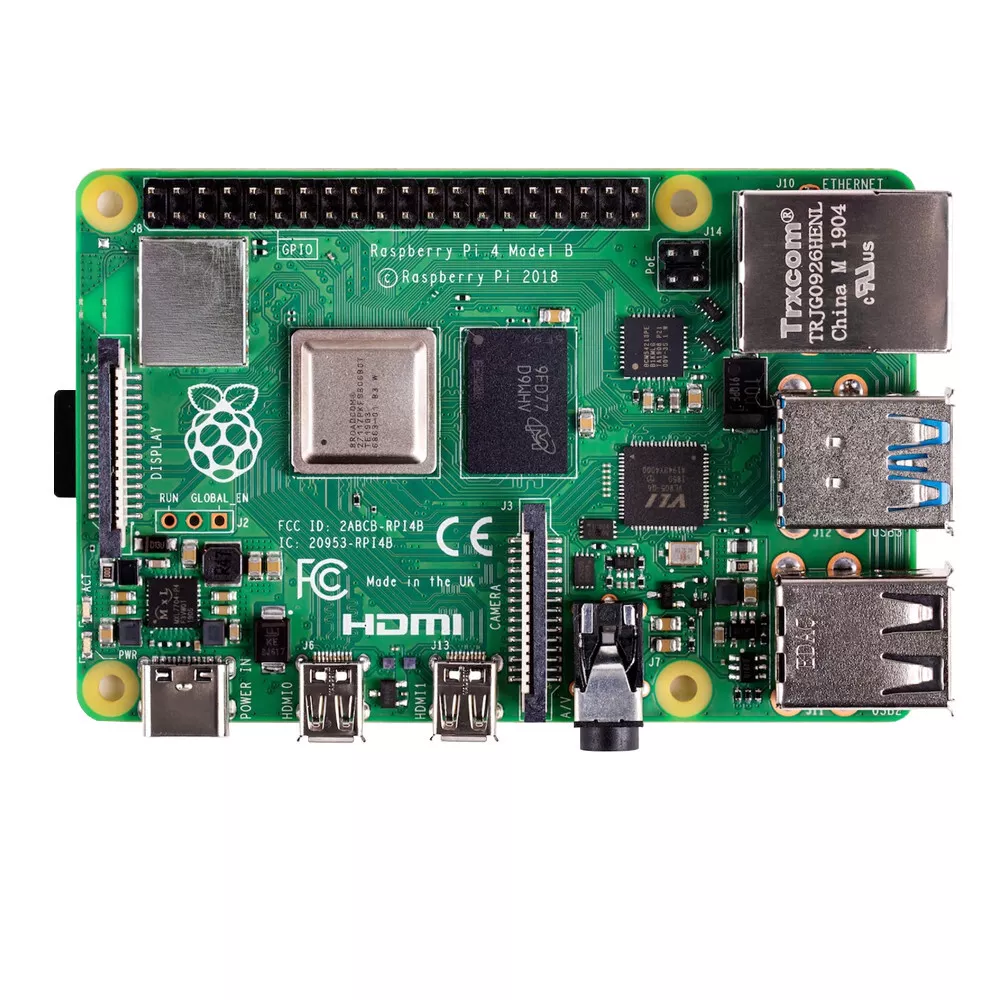
\includegraphics[width=0.3\textwidth]{figs/raspberrypi4.png}
    \caption{Raspberry Pi 4 - Unidad de control principal de la estación SatNOGS.}
    \label{fig:raspberry}
\end{figure}

\begin{figure}[H]
    \centering
    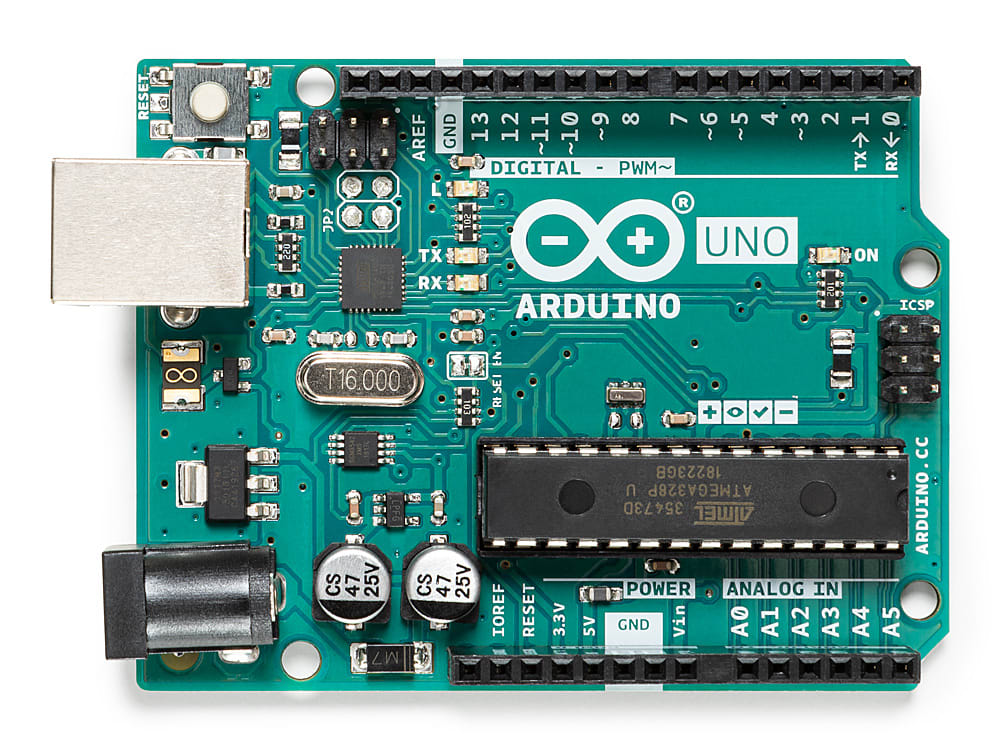
\includegraphics[width=0.3\textwidth]{figs/arduinounor3.png}
    \caption{Arduino UNO R3 - Encargado del sistema de monitoreo físico.}
    \label{fig:arduino}
\end{figure}

\begin{figure}[H]
    \centering
    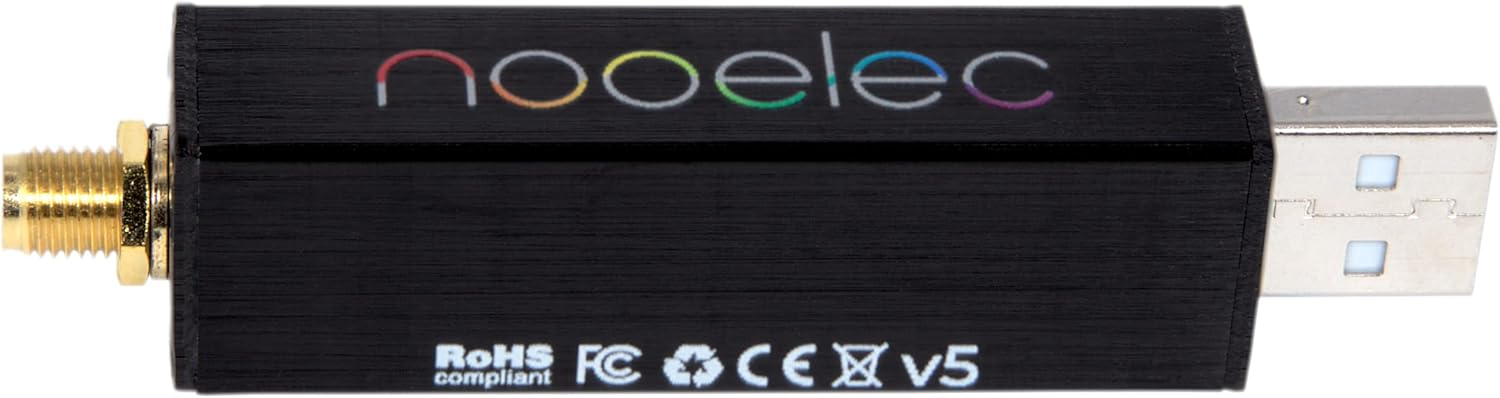
\includegraphics[width=0.3\textwidth]{figs/SDR Nooelec SMArt v5.png}
    \caption{SDR Nooelec SMArt v5 - Receptor de señales satelitales.}
    \label{fig:sdr}
\end{figure}

\begin{figure}[H]
    \centering
    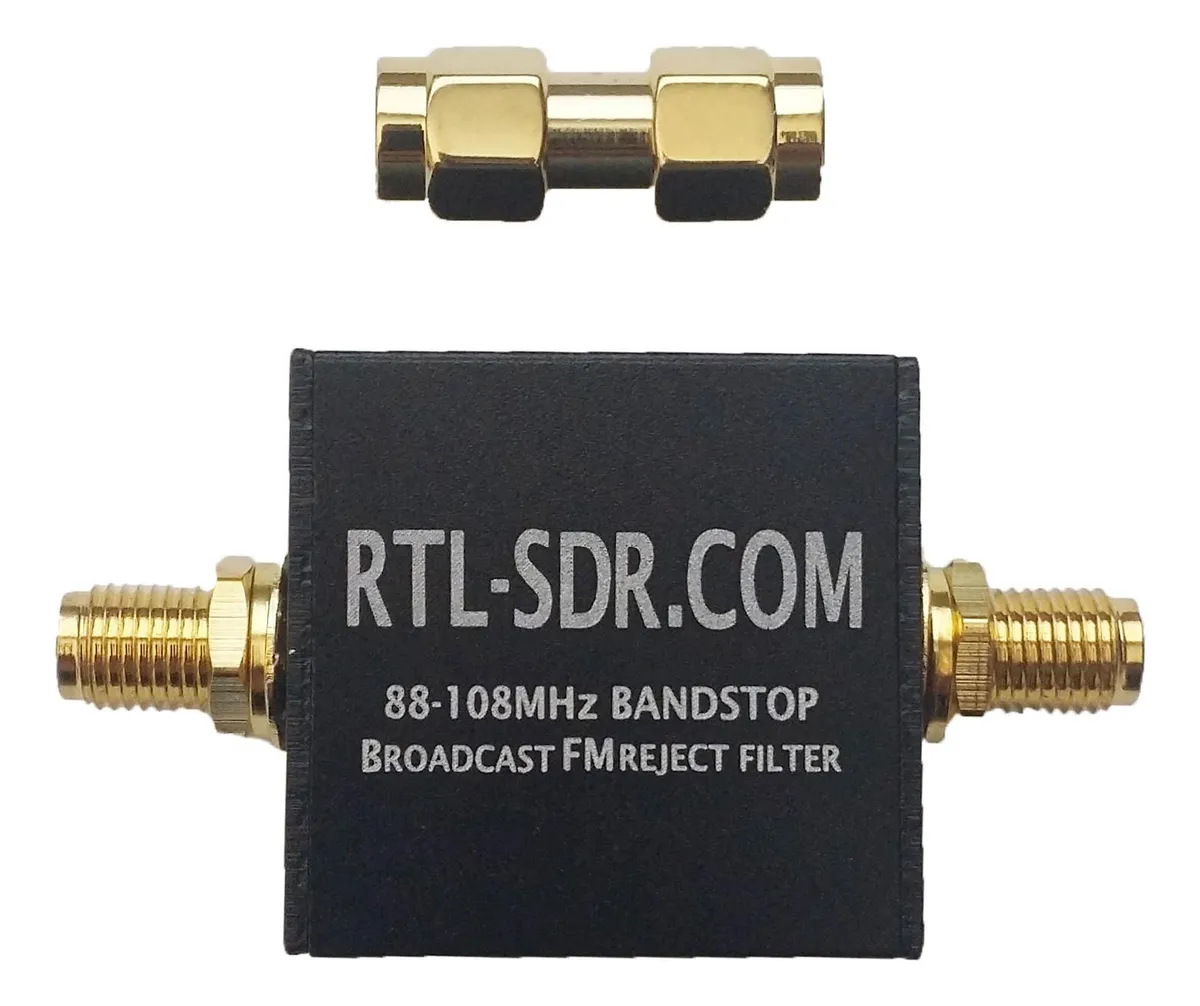
\includegraphics[width=0.3\textwidth]{figs/FMFilter.png}
    \caption{Filtro notch FM - Atenúa señales indeseadas de radio comercial.}
    \label{fig:filtro}
\end{figure}

\begin{figure}[H]
    \centering
    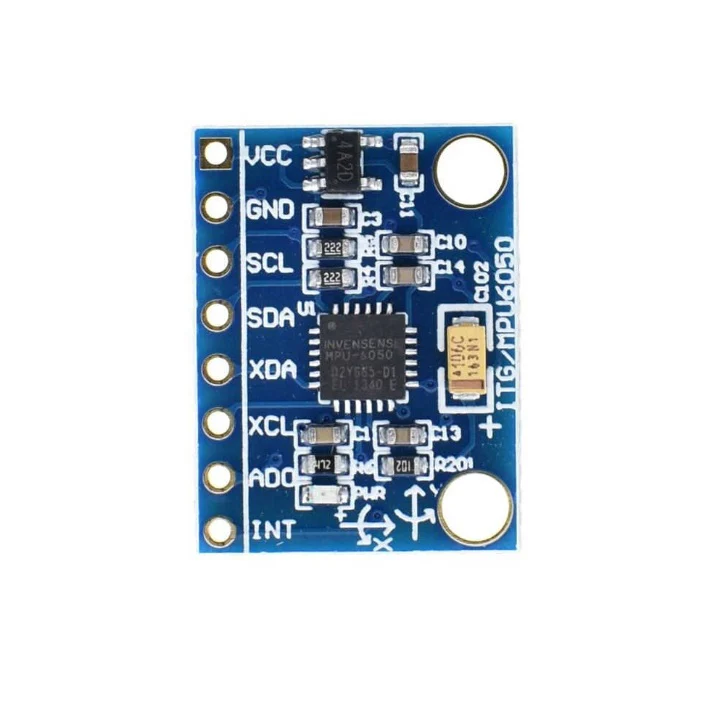
\includegraphics[width=0.25\textwidth]{figs/MPU6050.png}
    \caption{Sensor MPU6050 - Módulo de acelerómetro y giroscopio utilizado para detectar caídas, vibraciones y variaciones de orientación en la antena.}
    \label{fig:mpu6050}
\end{figure}

\begin{figure}[H]
    \centering
    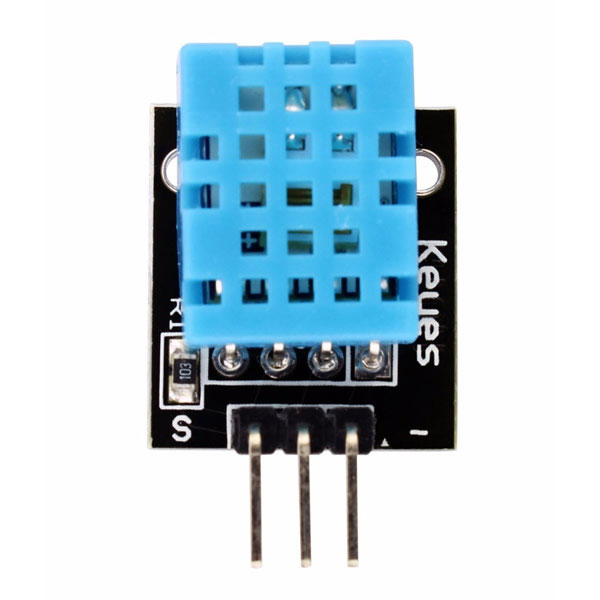
\includegraphics[width=0.25\textwidth]{figs/KY015.png}
    \caption{Sensor KY-015 - Sensor de temperatura y humedad utilizado para monitorear las condiciones ambientales que podrían afectar el hardware.}
    \label{fig:ky015}
\end{figure}

\begin{figure}[H]
    \centering
    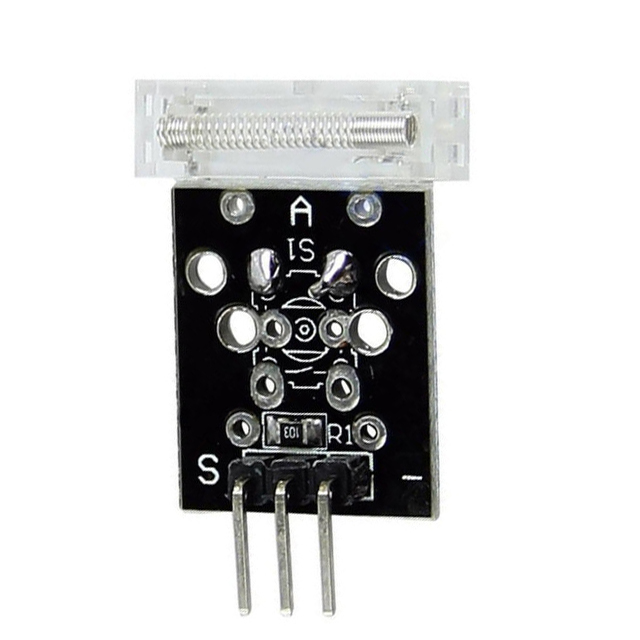
\includegraphics[width=0.25\textwidth]{figs/KY031.png}
    \caption{Sensor KY-031 - Sensor de impacto que permite detectar golpes o vibraciones fuertes, útiles para identificar eventos como impactos por aves o caídas del mástil.}
    \label{fig:ky031}
\end{figure}

\begin{figure}[H]
    \centering
    \includegraphics[width=0.42\textwidth]{figs/Turnstile.png}
    \caption{Antena Turnstile ensamblada y desplegada sobre trípode. Fabricada con varillas de aluminio y conectores coaxiales, esta configuración permite la recepción de señales satelitales en la banda VHF desde satélites de órbita baja (LEO).}
    \label{fig:antena_turnstile}
\end{figure}

\begin{figure}[H]
  \centering
  \includegraphics[width=0.75\linewidth]{figs/MonitorSetup.png}
  \caption{Sistema de monitoreo construido con Arduino, sensores KY y pantalla OLED. Todos los componentes están sujetos mediante bridas para garantizar la resiliencia y evitar desconexiones accidentales por vibraciones o impactos.}
  \label{fig:componentes_monitoreo}
\end{figure}

\section{Alcances del Proyecto}

El sistema desarrollado abarca dos componentes funcionales complementarios: un módulo de observación satelital automatizada basado en la red \textbf{SatNOGS}, y un módulo de monitoreo estructural y ambiental diseñado para asegurar la operatividad prolongada de la estación en condiciones adversas.

\subsection{Recepción y decodificación satelital con SatNOGS Client}

La estación incorpora una Raspberry Pi 4 que ejecuta la aplicación oficial \texttt{satnogs-client}, permitiendo su integración con la red global de observación colaborativa SatNOGS. Este cliente se comunica con los servidores centrales de la red y permite:

\begin{itemize}
    \item \textbf{Agendamiento y control de observaciones:} recepción automática de instrucciones para la captura de señales durante los pasos satelitales visibles desde la estación.
    \item \textbf{Captura de señales:} mediante un receptor SDR Nooelec V5 y un filtro de banda FM, se reciben señales en VHF/UHF de satélites meteorológicos, educativos o de telemetría.
    \item \textbf{Procesamiento local:} decodificación de señales (como APT o tramas digitales) con herramientas del ecosistema SatNOGS.
    \item \textbf{Contribución a la red:} subida automática de datos al repositorio SatNOGS, disponibles públicamente para investigación y educación.
\end{itemize}

\subsection{Monitoreo estructural y ambiental con Arduino}

Como complemento, se desarrolló un sistema embebido con un microcontrolador Arduino UNO R3 conectado a sensores ambientales y estructurales:

\begin{itemize}
    \item \textbf{MPU6050:} sensor de aceleración e inclinación para detectar caídas o cambios de orientación.
    \item \textbf{KY-031:} sensor de impacto o vibración para corroborar eventos físicos.
    \item \textbf{KY-015:} sensor de temperatura y humedad.
\end{itemize}

Estos sensores transmiten sus datos a la Raspberry Pi mediante el puerto serial. Una aplicación desarrollada en Python, denominada \texttt{MySatnogsMonitor}, permite:

\begin{itemize}
    \item \textbf{Emisión de alertas:} se genera una notificación si se detecta caída (cambio de orientación confirmado por impacto), si la temperatura supera los 32\textdegree C, o si la humedad supera el 90\%.
    \item \textbf{Prevención de fallos encubiertos:} se identifican situaciones en las que la estación parece conectada pero está operando con errores estructurales (como antenas caídas).
    \item \textbf{Visualización en tiempo real:} los datos se publican en un sitio web local accesible dentro de la red LAN de la estación.
\end{itemize}

Este diseño modular permite actuar proactivamente ante fallos físicos o ambientales, mejorando la confiabilidad de la estación y la calidad de los datos compartidos con la comunidad SatNOGS.


\section{Limitaciones del Proyecto}

A pesar de los avances logrados, el sistema desarrollado presenta varias limitaciones que abren oportunidades para futuras mejoras:

\begin{itemize}
    \item \textbf{Falta de demoduladores integrados:} actualmente, la estación captura datos en formato \texttt{.wav} (audio crudo) provenientes de los satélites, pero no cuenta con demoduladores específicos para misiones como NOAA (imágenes meteorológicas) o meteoros. Esto limita la utilidad directa de los datos para usuarios no especializados.
    
    \item \textbf{Protección ambiental:} aunque el sistema se encuentra funcional, los módulos electrónicos expuestos requieren coberturas resistentes al agua para soportar lluvias u otras condiciones climáticas adversas. Aún no se han implementado cajas o encapsulados impresos en 3D con esa finalidad.
    
    \item \textbf{Detección pasiva de lluvia:} el sistema actual no incluye un sensor dedicado a la detección de precipitaciones, lo cual reduciría la capacidad de anticipar eventos de riesgo para el hardware.
    
    \item \textbf{Rotación activa no implementada:} aunque la antena turnstile ha sido montada sobre un rodamiento con la intención de girarla cuando se detecte presencia de aves como mecanismo disuasorio, esta funcionalidad aún no ha sido implementada.
    
    \item \textbf{Ubicación subóptima para observación astronómica:} si bien la estación cumple con su objetivo funcional, sería ideal replicar este modelo en ubicaciones geográficas más estratégicas —como zonas de alta altitud o con amplio campo de visibilidad no interrumpido— para maximizar la cobertura de pasos satelitales y mejorar la calidad de las observaciones.
    
    \item \textbf{Falta de integración en PCB:} actualmente, el sistema está construido sobre protoboard y conexiones modulares, lo que lo hace funcional pero menos robusto ante vibraciones o manipulación. Sería ideal que, en futuras versiones, se proponga un diseño de placa de circuito impreso (PCB) que permita miniaturizar y consolidar el sistema, facilitando tanto su replicación como su despliegue en ambientes más exigentes.
\end{itemize}



\section{Desarrollo}

\subsection{Hardware del Proyecto}

La antena utilizada en este proyecto es una \textbf{antena turnstile}, diseñada específicamente para la recepción de satélites meteorológicos en la banda VHF (137.5 MHz), tales como NOAA-15, 18 y 19. 

El diseño replicado está basado en el esquema desarrollado por el radioaficionado italiano I6IBE, ampliamente utilizado por la comunidad de entusiastas por su simplicidad y rendimiento confiable~\cite{i6ibe_turnstile}. 

Este diseño se compone de dos dipolos cruzados, con elementos reflectores por debajo de cada uno, generando una polarización circular RHCP adecuada para la recepción de señales provenientes de satélites de órbita baja. Las dimensiones de los dipolos y transformadores de impedancia están calculadas para asegurar una adaptación efectiva a 52 ohmios. La Figura~\ref{fig:antena_i6ibe} presenta el esquema técnico replicado en el presente proyecto.

\begin{figure}[H]
\centering
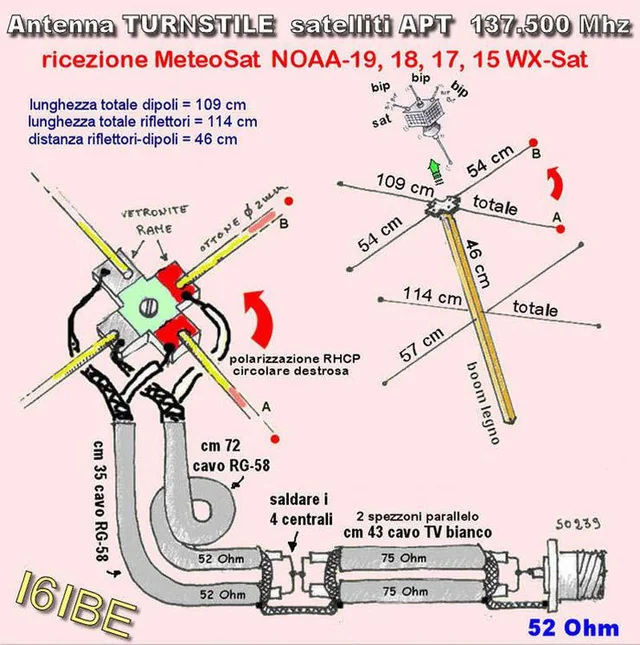
\includegraphics[width=0.95\linewidth]{figs/turnstile_i6ibe.png}
\caption{Diseño técnico de la antena turnstile para satélites APT (I6IBE). Fuente:~\cite{i6ibe_turnstile}}
\label{fig:antena_i6ibe}
\end{figure}




El sistema desarrollado se compone de múltiples sensores conectados a una placa \textbf{Arduino Uno R3}, la cual actúa como unidad de adquisición de datos. Esta placa se comunica mediante una conexión serial con una \textbf{Raspberry Pi 4}, que cumple funciones de procesamiento, visualización remota y transmisión de eventos críticos.



\begin{figure}[H]
  \centering
  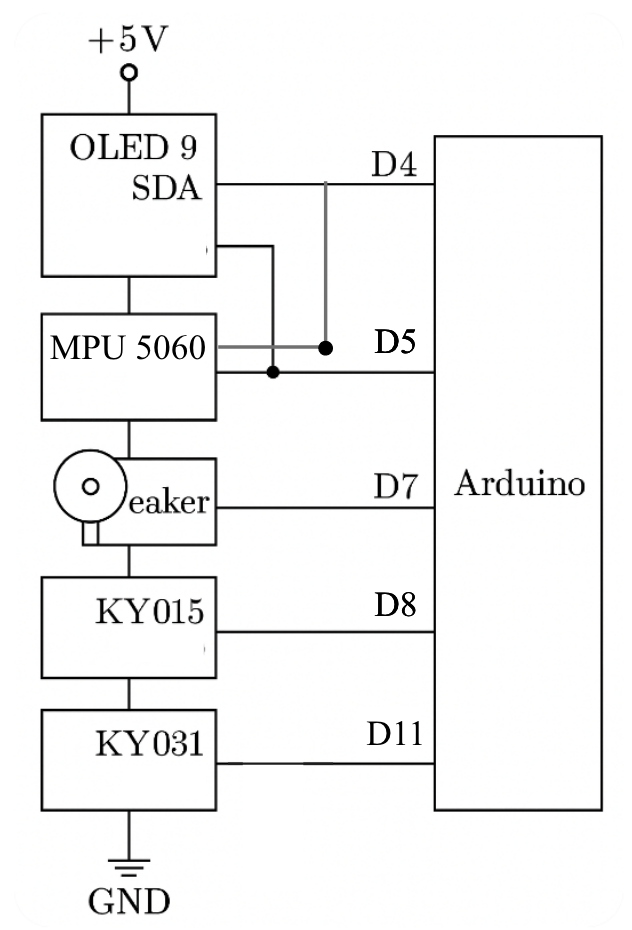
\includegraphics[width=0.55\linewidth]{figs/Esquema.png}
  \caption{Esquema de conexión de los componentes del sistema.}
  \label{fig:esquema_conexion}
\end{figure}


\begin{itemize}
  \item \textbf{MPU6050 (Acelerómetro y Giroscopio)}: Conectado por interfaz I2C a los pines A4 (SDA) y A5 (SCL).
  \item \textbf{DHT11 (Temperatura y Humedad - Módulo KY-015)}: Conectado al pin digital D8.
  \item \textbf{Sensor de impacto KY-031}: Conectado al pin digital D11.
  \item \textbf{Pantalla OLED 0.91"}: También conectada por I2C (SDA y SCL compartidos con MPU6050).
\end{itemize}


\subsection{Software del Proyecto}

El sistema de monitoreo se basa en una arquitectura distribuida entre dos componentes principales:

\begin{itemize}
  \item \textbf{Arduino Uno R3}: Encargado de la lectura periódica de sensores y envío de eventos por comunicación serial.
  \item \textbf{Raspberry Pi 4}: Responsable de procesar los datos, emitir notificaciones, y recolectar información satelital mediante SDR.
\end{itemize}

Para facilitar la mantenibilidad del código, se empleó una estructura modular implementada sobre \texttt{PlatformIO}, dividiendo el sistema en carpetas por funcionalidades:

\begin{itemize}
  \item \texttt{display/OledDisplay.h}: Control de la pantalla OLED (mediante \texttt{Adafruit\_SSD1306}).
  \item \texttt{sensors/Accelerometer.h}: Abstracción del MPU6050 (mediante \texttt{Wire}).
  \item \texttt{sensors/TempHumiditySensor.h}: Manejo del DHT11 (utilizando \texttt{DHT.h}).
  \item \texttt{sensors/ImpactSensor.h}: Lectura digital del sensor de impacto KY-031.
\end{itemize}

Se utilizó el protocolo I2C para la comunicación con los sensores digitales compartidos (OLED y MPU6050), y señales digitales simples para los sensores KY. La comunicación entre Arduino y Raspberry Pi se realiza mediante puerto serial USB.

Todo el material complementario del proyecto, incluyendo el código fuente, diagramas electrónicos, archivos STL para impresión 3D, documentación técnica y videos demostrativos, se encuentra disponible en el repositorio oficial del proyecto: \url{https://github.com/joelibaceta/resilient-turnstile}. Este repositorio permite la reproducción, adaptación y mejora de la solución propuesta por parte de otros desarrolladores o instituciones educativas interesadas en implementar estaciones SatNOGS con capacidad de monitoreo estructural autónomo.

\subsubsection{Código Principal en Arduino}

A continuación se muestra un extracto del archivo \texttt{main.cpp}:

\begin{lstlisting}[language=C++, caption={Fragmento de código fuente de Arduino}, label={lst:arduino_code}, basicstyle=\ttfamily\small, breaklines=true]
#include <Arduino.h>
#include "display/OledDisplay.h"
#include "sensors/Accelerometer.h"
#include "sensors/TempHumiditySensor.h"
#include "sensors/ImpactSensor.h"

#define BUZZER_PIN 7

OledDisplay oled;
Accelerometer imu;
TempHumiditySensor dht(8);
ImpactSensor impact(11);

void setup() {
  Serial.begin(115200);
  Wire.begin();
  pinMode(BUZZER_PIN, OUTPUT);
  digitalWrite(BUZZER_PIN, LOW);
  oled.begin(); imu.begin(); dht.begin(); impact.begin();
  oled.showMessage("Sistema iniciado");
  Serial.println("EVENT,system_ready");
}
\end{lstlisting}

\subsubsection{Formato de Salida Serial y Bucle Principal}

El bucle principal está diseñado para emitir mensajes por el puerto serial en un formato estructurado y legible por el sistema en Raspberry Pi. Este escucha los eventos y métricas usando etiquetas como \texttt{EVENT} y \texttt{METRIC} para diferenciarlos.

\begin{itemize}
  \item \texttt{EVENT,...} indica la detección de sucesos relevantes (como impacto).
  \item \texttt{METRIC,...} reporta variables continuas como temperatura, humedad o aceleración.
\end{itemize}

Este formato facilita la integración con herramientas en Raspberry Pi que procesan los datos y disparan acciones o alertas.

\begin{lstlisting}[language=C++, caption={Bucle principal y salida serial para integración con Raspberry Pi}, label={lst:arduino_loop}, basicstyle=\ttfamily\small, breaklines=true]
void loop() {
  oled.clear();

  // Evento: impacto
  if (impact.isTriggered()) {
    Serial.println("EVENT,impact_detected");
    oled.printFormatted("Impacto detectado");
    digitalWrite(BUZZER_PIN, HIGH);
    delay(500);
    digitalWrite(BUZZER_PIN, LOW);
    delay(1000);
  }

  // Métricas: acelerómetro y giroscopio
  float ax, ay, az, gx, gy, gz;
  if (imu.readAccel(ax, ay, az) && imu.readGyro(gx, gy, gz)) {
    Serial.printf("METRIC,accel_x=%.2f,accel_y=%.2f,accel_z=%.2f\n", ax, ay, az);
    Serial.printf("METRIC,gyro_x=%.2f,gyro_y=%.2f,gyro_z=%.2f\n", gx, gy, gz);
    oled.printFormatted("Acel:\nX=%.2fg\nY=%.2fg\nZ=%.2fg", ax, ay, az);
  }

  delay(1000);
  oled.clear();

  // Métricas: temperatura y humedad
  float t, h;
  if (dht.read(t, h)) {
    Serial.printf("METRIC,temp=%.1f,hum=%.1f\n", t, h);
    oled.printFormatted("T:%.1f", t);
    oled.printFormatted("H:%.1f", h);
    delay(2000);
  }

  delay(1000);
}
\end{lstlisting}



\section{Pruebas de Validación}

\subsection{Procedimiento de Validación}

Para validar el funcionamiento del sistema desarrollado, se realizó un despliegue completo en condiciones reales EN lIMA. La estación, identificada en la red SatNOGS como \textbf{Nodo 4121 - Lima Node}, fue equipada con una antena turnstile VHF, sensores de monitoreo estructural y ambiental, un receptor SDR, y los módulos software mencionados anteriormente.

Las pruebas se enfocaron en dos objetivos principales:

\begin{itemize}
  \item Validar la capacidad de la estación para realizar observaciones satelitales reales dentro de la red colaborativa SatNOGS.
  \item Verificar que el sistema de monitoreo físico (impacto, temperatura y aceleración) permite detectar condiciones anómalas y reaccionar ante ellas de manera proactiva.
\end{itemize}



\subsection{Resultados Cuantificables y Observaciones}

Durante el periodo de prueba, la estación permanece activa por más de tres semanas continuas. En ese tiempo, se registraron \textbf{175 observaciones programadas}, muchas de las cuales permitieron la captura de telemetría útil desde satélites de órbita baja. La Figura~\ref{fig:resumen_satnogs} muestra el estado actual del nodo dentro de la plataforma SatNOGS, incluyendo su ubicación geográfica, tipo de antena, tasa de éxito y cantidad de observaciones realizadas.


\begin{figure}[H]
  \centering
  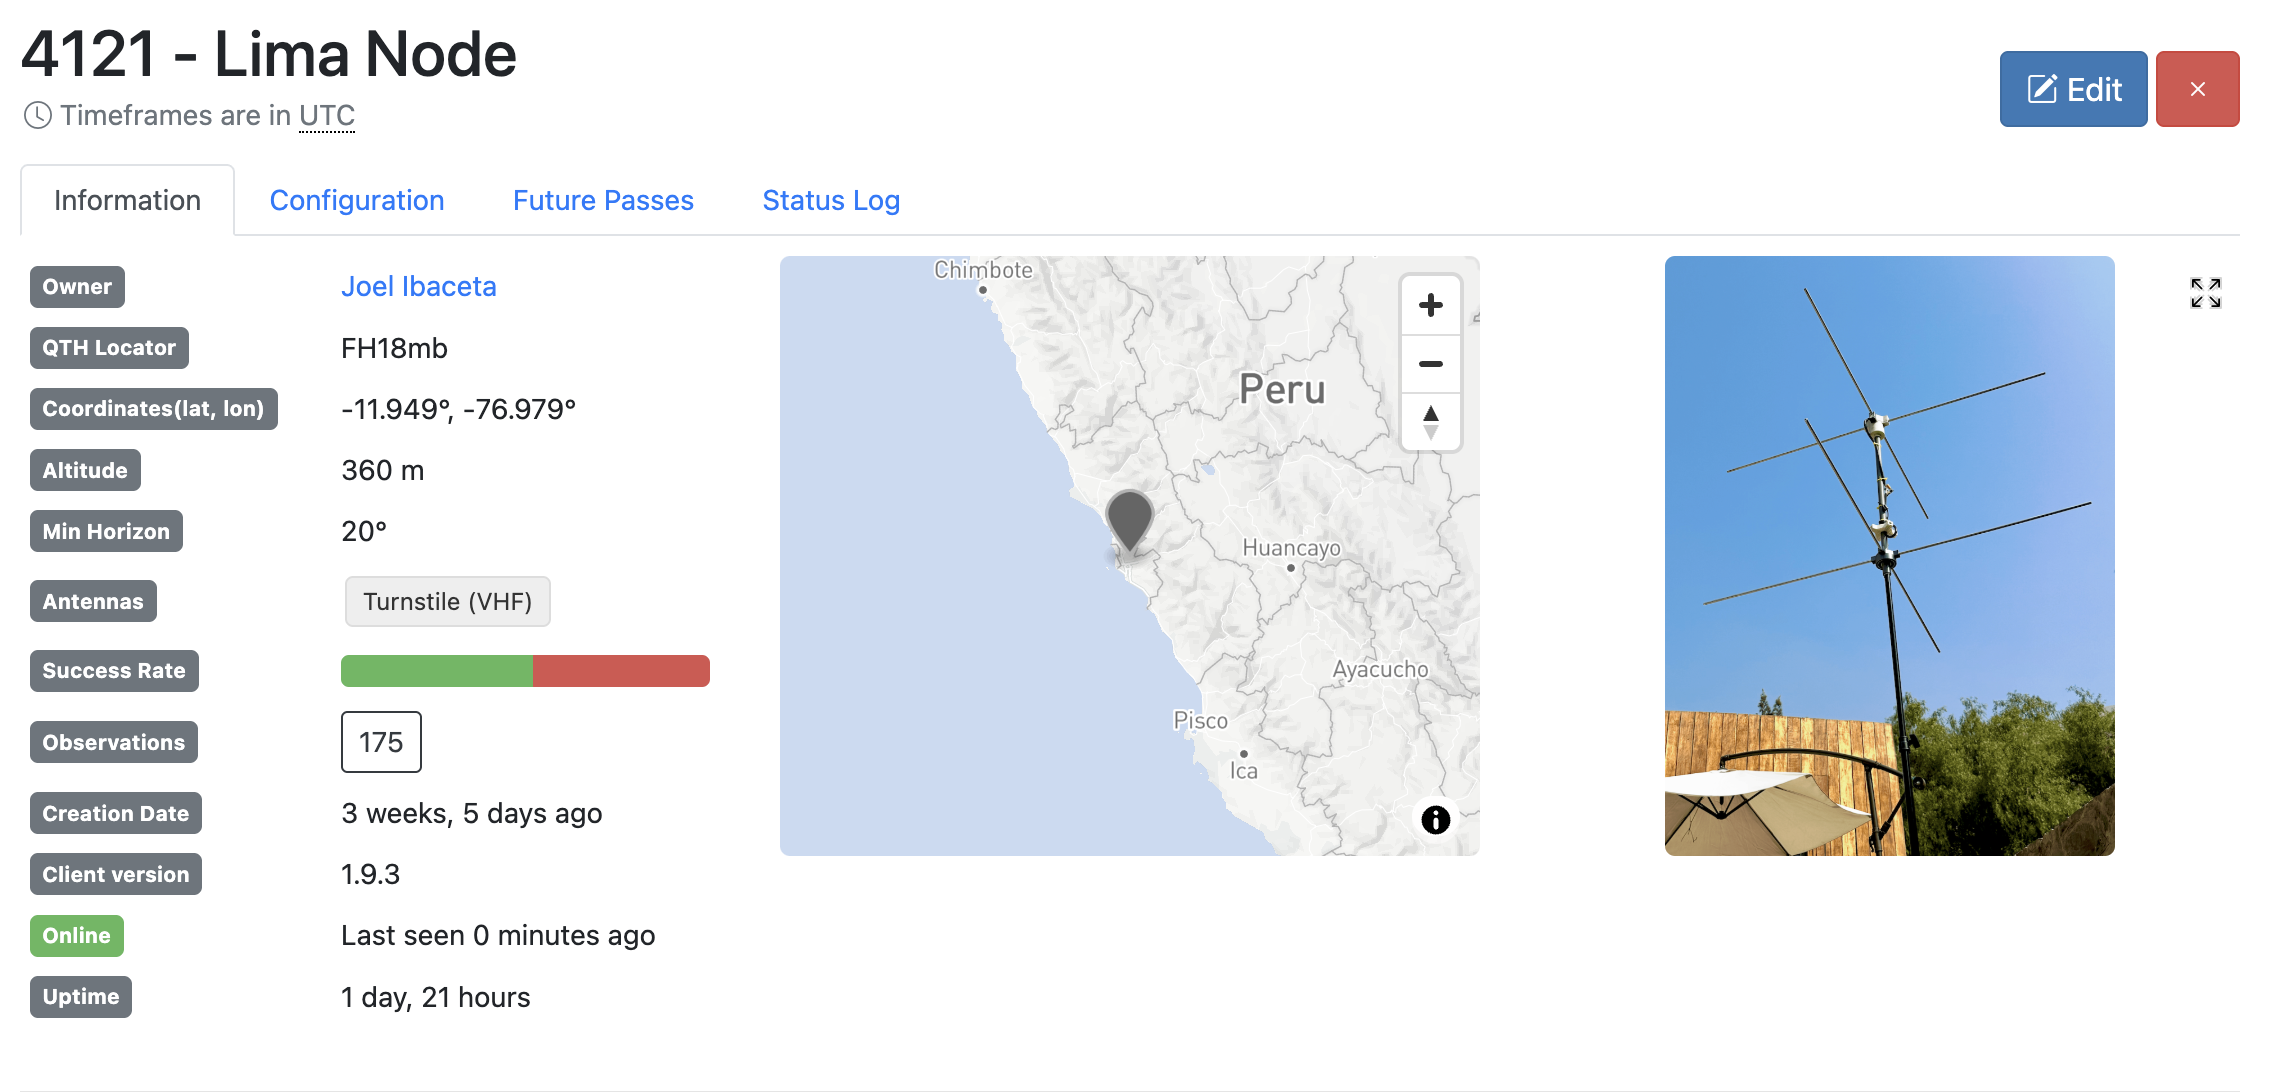
\includegraphics[width=0.95\linewidth]{figs/4121_Node.png}
  \caption{Resumen técnico del nodo 4121 – Lima Node, activo en la red SatNOGS.}
  \label{fig:resumen_satnogs}
\end{figure}

La estación desarrollada puede ser consultada públicamente en la red SatNOGS bajo el identificador \textbf{4121 - Lima Node}. Su historial de actividad, observaciones realizadas, tasa de éxito y registros de uso por parte de otros operadores están disponibles en tiempo real en la siguiente dirección: \url{https://network.satnogs.org/stations/4121}.

El nodo fue utilizado por otros miembros de la comunidad internacional para capturar telemetría satelital. La Figura~\ref{fig:telemetria_lapan} documenta una observación exitosa del satélite LAPAN-A2 por parte de Fredy Damkalis, miembro del equipo central de la red SatNOGS, utilizando la estación de Lima para recuperar información transmitida por el satélite.

\begin{figure}[H]
  \centering
  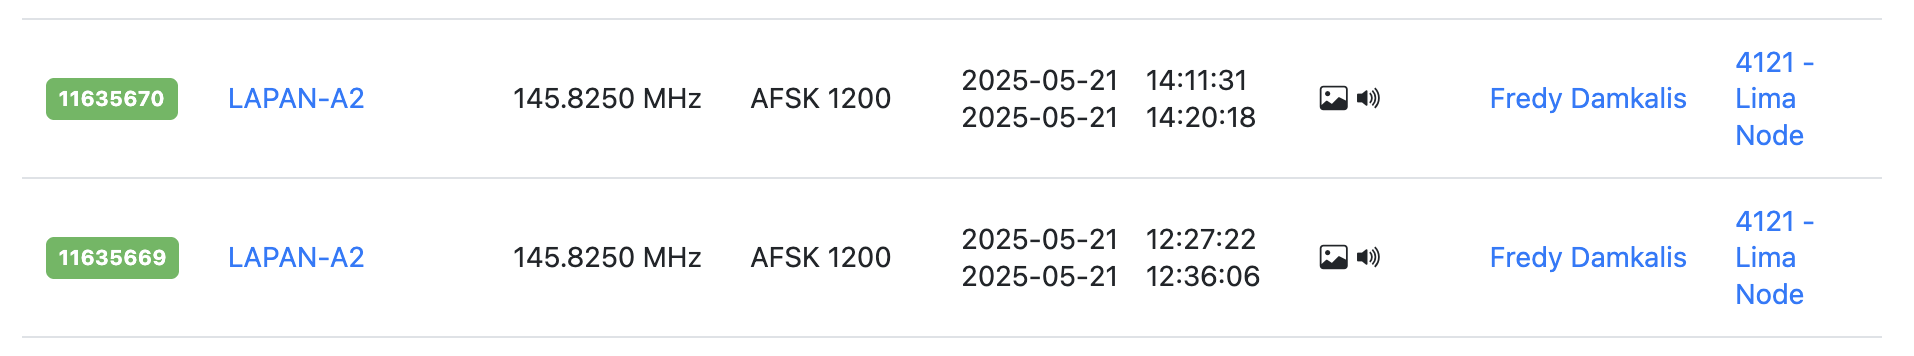
\includegraphics[width=1\linewidth]{figs/observacion_fredy.png}
  \caption{Observación exitosa del satélite LAPAN-A2 a través del nodo 4121.}
  \label{fig:telemetria_lapan}
\end{figure}

\subsection{Eventos de Fallo y Mejora de Resiliencia}

Durante el periodo de pruebas también se registró un incidente real de caída de la antena, ocasionado por un ave que se posó sobre una de las varillas, desestabilizando la estructura. Este evento permitió validar la utilidad del sistema de monitoreo estructural: la caída fue detectada por el acelerómetro y el sensor de impacto, generando una alerta temprana.

En ausencia de este sistema, la estación habría continuado enviando observaciones fallidas a la red. De hecho, como se muestra en la Figura~\ref{fig:FailObservations}, antes de implementar la respuesta activa, el nodo seguía en estado “online” pero generaba observaciones vacías o completamente oscuras, afectando la calidad de datos. A la derecha se observa el estado tras implementar la lógica de apagado remoto mediante un enchufe inteligente controlado por comandos de voz (Alexa), lo que evita que la estación reciba nuevas tareas hasta que su integridad física sea verificada.

\begin{figure}[H]
  \centering
  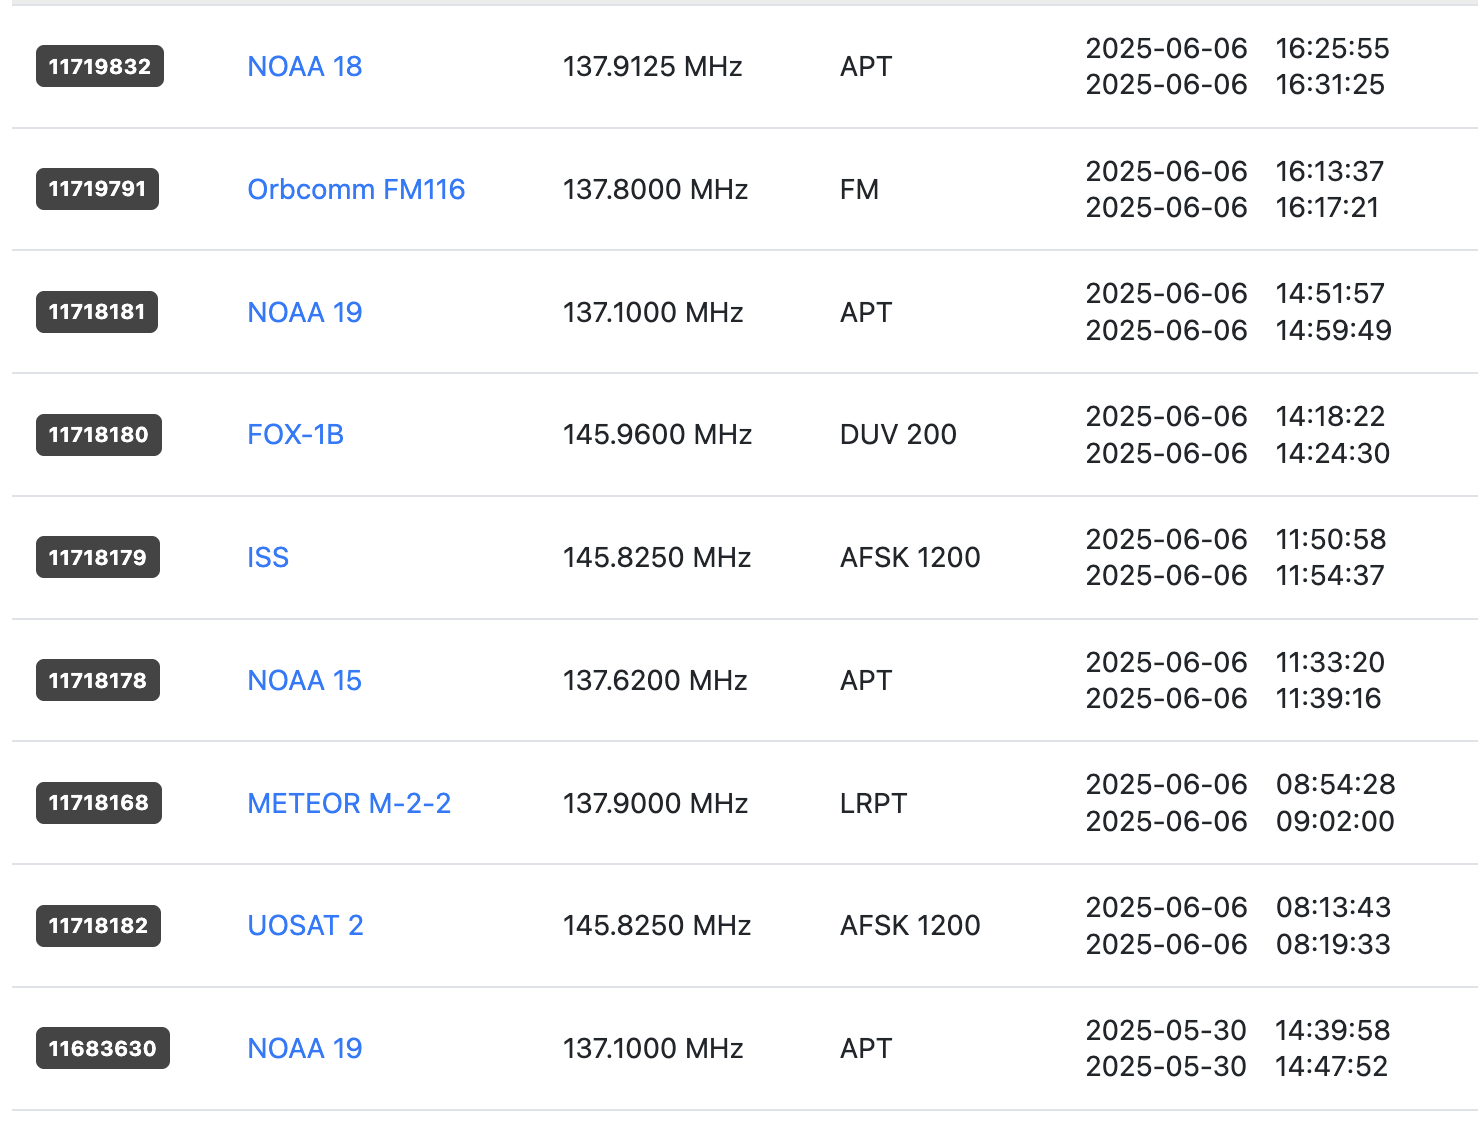
\includegraphics[width=0.85\linewidth]{figs/FailObservations.png}
  \caption{Observaciones fallidas, debido a evento de caida no detectado a tiempo}
  \label{fig:FailObservations}
\end{figure}

Este mecanismo de respuesta remota contribuye a mejorar la \textbf{resiliencia operativa} de la estación, permitiendo suspender temporalmente el nodo y evitar que la comunidad reciba datos erróneos, optimizando el uso de recursos y reforzando la confiabilidad de la red SatNOGS.

\section{Conclusiones y Recomendaciones}

\subsection{Conclusiones}

\textbf{Objetivo 1: Desarrollar un sistema de adquisición de datos con sensores físicos conectado a una placa Arduino Uno.}

Se implementó un sistema funcional compuesto por un acelerómetro (MPU6050), un sensor de impacto (KY-031), un sensor de temperatura y humedad (KY-015) y una pantalla OLED. El sistema mantuvo un funcionamiento continuo y estable durante un periodo de tres semanas, permitiendo la detección efectiva de eventos físicos como impactos y variaciones de aceleración. 

\vspace{0.5em}
\textbf{Objetivo 2: Desarrollar un sistema de monitoreo capaz de emitir eventos y métricas vía puerto serial para ser interpretados por un proceso externo.}

El microcontrolador Arduino transmitió correctamente los eventos en formato estructurado a través del puerto serial, permitiendo su interpretación por un sistema externo basado en Raspberry Pi 4. Se verificó la correcta lectura, interpretación y uso de dichas métricas en un entorno operativo, incluyendo el disparo de acciones remotas. 

\vspace{0.5em}
\textbf{Objetivo 3: Validar el funcionamiento de la estación SatNOGS en condiciones reales con soporte de monitoreo estructural.}

La estación SatNOGS (nodo 4121) se mantuvo operativa durante más de tres semanas, generando más de 175 observaciones. Se documentó su utilización por parte de usuarios externos a la institución, incluyendo la decodificación de telemetría del satélite LAPAN-A2. Además, se evitó la generación de observaciones fallidas gracias al sistema de monitoreo estructural, lo cual demuestra su aporte directo a la resiliencia operativa del nodo. Por lo tanto, el objetivo fue cumplido con resultados cuantificables.

\subsection{Recomendaciones}

Durante el desarrollo e implementación del sistema, se identificaron una serie de oportunidades de mejora que podrían ser consideradas en trabajos futuros o al replicar el proyecto en otras estaciones SatNOGS:

\begin{itemize}
  \item \textbf{Protección estructural de los componentes electrónicos:} Se recomienda diseñar e imprimir una carcasa resistente a la intemperie para los módulos sensores y la placa Arduino. La instalación actual, si bien funcional, requiere protección adicional frente a humedad, polvo y radiación solar directa.

  \item \textbf{Incorporación de sensor de lluvia:} Para aumentar la cobertura de eventos ambientales, sería beneficioso integrar un sensor de precipitación que permita anticipar posibles riesgos eléctricos o estructurales, y suspender temporalmente la operación.

  \item \textbf{Automatización del apagado preventivo:} El sistema actualmente requiere intervención manual para ejecutar el apagado remoto mediante dispositivos domóticos. Se sugiere automatizar esta lógica en la Raspberry Pi, de modo que ante condiciones críticas el apagado se ejecute de forma autónoma sin depender del usuario.

  \item \textbf{Demodulación automática de señales:} Actualmente las señales recibidas se almacenan en formato WAV sin procesamiento posterior. Sería recomendable integrar herramientas como \texttt{noaa-apt}, \texttt{meteor-demod} u otros paquetes compatibles para la generación automática de imágenes meteorológicas y productos científicos.

  \item \textbf{Diseño de una PCB dedicada:} El uso de protoboard y cables sueltos limita la robustez del sistema. El diseño de una placa de circuito impreso (PCB) permitiría miniaturizar, estabilizar y estandarizar el hardware, facilitando la producción de réplicas funcionales.

  \item \textbf{Instalación en ubicaciones estratégicas:} Si bien la estación en Lima ha sido efectiva, se recomienda considerar futuras instalaciones en zonas más elevadas o con menor interferencia electromagnética, como áreas rurales, zonas de montaña o campus universitarios con cielos despejados. Esto aumentaría la calidad de recepción y la relevancia científica de las observaciones.
\end{itemize}

\begin{thebibliography}{9}

\bibitem{julien2021satnogs}
N.~Julien, A.~Tsioliaridou, and E.~Kotsakis, 
``SatNOGS: Towards a Modern, Crowd-Sourced and Open Network of Ground Stations,'' 
in \textit{Proc. IEEE Aerospace Conf.}, 2021.

\bibitem{gayoso2019estacion}
F.~Gayoso, S.~Melgarejo, and F.~Mullukian, 
``Construcción y operación de estación terrena para el seguimiento de satélites,'' 
Facultad de Ingeniería, Universidad de la República, 2019. 
[En línea]. Disponible en: \url{https://www.fing.edu.uy}

\bibitem{argentina2020balcarce}
``Estación terrena en Balcarce y Córdoba,'' 2020. 
[En línea]. Disponible en: \url{https://lu4aao.org/satelites.htm}

\bibitem{i6ibe_turnstile}
I6IBE, “Antenna TURNSTILE satelliti APT 137.500 MHz,” diseño publicado en foros de radioaficionados. Disponible en: \url{https://www.i6ibe.it/turnstile.htm} [Accedido: 07-jun-2025].

\bibitem{ibaceta2025turnstile}
J. Ibaceta, “\textit{Resilient Turnstile: Sensor-Enhanced Passive Antenna for Satellite and Environmental Monitoring},” GitHub, 2025. [En línea]. Disponible en: \url{https://github.com/joelibaceta/resilient-turnstile}. [Accedido: 7-jun-2025].

\end{thebibliography}

\end{document}